\documentclass{article}
\usepackage[utf8]{inputenc}
\usepackage{listings}
\usepackage{multimedia} % to embed movies in the PDF file
\usepackage{graphicx}
\usepackage{comment}
\usepackage[english]{babel}
\usepackage{amsmath}
\usepackage{amsfonts}
\usepackage{wrapfig}
\usepackage{multirow}
\usepackage{verbatim}
\usepackage{float}
\usepackage{cancel}
\usepackage{caption}
\usepackage{subcaption}
%!TEX root = main.tex



\newcommand{\eref}[1]{\mbox{\rm(\ref{#1})}}
\newcommand{\tref}[1]{\mbox{\rm\ref{#1}}}
\newcommand{\set}[2]{\left\{ #1 \; : \; #2 \right\} }
\newcommand{\deq}{\raisebox{0pt}[1ex][0pt]{$\stackrel{\scriptscriptstyle{\rm def}}{{}={}}$}}

\newcommand {\DS} {\displaystyle}

\newcommand{\real}{\mathbb{R}}



\newcommand {\half} {\mbox{$\frac{1}{2}$}}
\newcommand{\force}{{\mathbf{f}}}
\newcommand{\strain}{{\boldsymbol{\varepsilon}}}
\newcommand{\stress}{{\boldsymbol{\sigma}}}
\renewcommand{\div}{{\boldsymbol{\nabla}}}

\newcommand {\cA} {{\cal A}}
\newcommand {\cB} {{\cal B}}
\newcommand {\cC} {{\cal C}}
\newcommand {\cD} {{\cal D}}
\newcommand {\cE} {{\cal E}}
\newcommand {\cK} {{\cal K}}
\newcommand {\cL} {{\cal L}}
\newcommand {\cP} {{\cal P}}
\newcommand {\cQ} {{\cal Q}}
\newcommand {\cR} {{\cal R}}
\newcommand {\cV} {{\cal V}}
\newcommand {\cW} {{\cal W}}
\newcommand {\CC} {{\cal C}}
\newcommand {\CD} {{\cal D}}
\newcommand {\CH} {{\cal H}}
\newcommand {\CS} {{\cal S}}
\newcommand {\CU} {{\cal U}}
\newcommand {\CY} {{\cal Y}}



\newcommand{\bzero}{\mathbf{0}}
\newcommand{\ba}{\mathbf{a}}
\newcommand{\bb}{\mathbf{b}}
\newcommand{\bc}{\mathbf{c}}
\newcommand{\bd}{\mathbf{d}}
\newcommand{\be}{\mathbf{e}}
\newcommand{\bg}{\mathbf{g}}
\newcommand{\bh}{\mathbf{h}}
\newcommand{\bl}{\mathbf{l}}
\newcommand{\bn}{\mathbf{n}}
\newcommand{\bp}{\mathbf{p}}
\newcommand{\bq}{\mathbf{q}}
\newcommand{\br}{\mathbf{r}}
\newcommand{\bs}{\mathbf{s}}
\newcommand{\bt}{\mathbf{t}}
\newcommand{\bu}{\mathbf{u}}
\newcommand{\bv}{\mathbf{v}}
\newcommand{\bw}{\mathbf{w}}
\newcommand{\bx}{\mathbf{x}}
\newcommand{\by}{\mathbf{y}}
\newcommand{\bz}{\mathbf{z}}
\newcommand{\bA}{{\mathbf A}}
\newcommand{\bB}{\mathbf{B}}
\newcommand{\bC}{\mathbf{C}}
\newcommand{\bD}{\mathbf{D}}
\newcommand{\bE}{\mathbf{E}}
\newcommand{\bF}{\mathbf{F}}
\newcommand{\bG}{\mathbf{G}}
\newcommand{\bH}{\mathbf{H}}
\newcommand{\bI}{\mathbf{I}}
\newcommand{\bJ}{\mathbf{J}}
\newcommand{\bK}{\mathbf{K}}
\newcommand{\bL}{\mathbf{L}}
\newcommand{\bM}{\mathbf{M}}
\newcommand{\bN}{\mathbf{N}}
\newcommand{\bO}{\mathbf{O}}
\newcommand{\bP}{\mathbf{P}}
\newcommand{\bQ}{\mathbf{Q}}
\newcommand{\bR}{\mathbf{R}}
\newcommand{\bS}{\mathbf{S}}
\newcommand{\bU}{\mathbf{U}}
\newcommand{\bV}{\mathbf{V}}
\newcommand{\bW}{\mathbf{W}}
\newcommand{\bX}{\mathbf{X}}
\newcommand{\bY}{\mathbf{Y}}
\newcommand{\bZ}{\mathbf{Z}}

\newcommand{\bgamma}{{\boldsymbol{\gamma}}}
\newcommand{\bmu}{{\boldsymbol{\mu}}}
\newcommand{\bkappa}{{\boldsymbol{\kappa}}}
\newcommand{\blambda}{{\boldsymbol{\lambda}}}
\newcommand{\bLambda}{{\boldsymbol{\Lambda}}}
\newcommand{\bpi}{{\boldsymbol{\pi}}}
\newcommand{\bPi}{{\boldsymbol{\Pi}}}
\newcommand{\btheta}{{\boldsymbol{\theta}}}
\newcommand{\bTheta}{{\boldsymbol{\Theta}}}
\newcommand{\bSigma}{{\boldsymbol{\Sigma}}}






\title{AMATH 585 Assignment 7}
\author{Cade Ballew}
\date{March 9, 2022}

\begin{document}
	
\maketitle
	
\section{Problem 1}
Consider the conjugate gradient algorithm 
\vspace{.1in}

\begin{center}
\begin{tabular}{|l|} \hline
Given $x_0$, compute $r_0 = b - A x_0$, and set $p_0 = r_0$. \\
For $k=1,2, \ldots$, \\
$~~$ Compute $A p_{k-1}$. \\
$~~$ Set $x_k = x_{k-1} + a_{k-1} p_{k-1}$, where $a_{k-1} = \frac{\langle r_{k-1} , r_{k-1} \rangle}
{\langle p_{k-1} , A p_{k-1} \rangle}$. \\
$~~$ Compute $r_k = r_{k-1} - a_{k-1} A p_{k-1}$. \\
$~~$ Set $p_k = r_k + b_{k-1} p_{k-1}$, where $b_{k-1} = \frac{\langle r_k , r_k \rangle}
{\langle r_{k-1} , r_{k-1} \rangle}$. \\
Endfor \\ \hline
\end{tabular}
\end{center}
\vspace{.1in}
where $A$ is symmetric and positive definite. We wish to use induction on $k$ to show that the residual vectors $r_0 , \ldots , r_k$ are orthogonal to each other
($\langle r_i , r_j \rangle = 0$ if $i \neq j$) and that the direction vectors 
$p_0 , \ldots , p_k$ are $A$-orthogonal ($\langle p_i , A p_j \rangle = 0$ if $i \neq j$).\\
First, it is important to note that because $A$ is symmetric,
\[
\ip{v}{Av}=v^*Av=v^*A^*v=(Av)^*v=\ip{Av}{v}
\]
for any vector $v$ of appropriate dimension. Now, as a base case, observe that because $r_0=p_0$, 
\begin{align*}
\ip{r_1}{r_0}&=\ip{r_0-a_0Ar_0}{r_0}=\ip{r_0}{r_0}-a_0\ip{Ar_0}{r_0}=\ip{r_0}{r_0}-\frac{\ip{r_0}{r_0}}{\ip{p_0}{Ap_0}}\ip{Ar_0}{r_0}\\&=\ip{r_0}{r_0}-\frac{\ip{r_0}{r_0}}{\ip{r_0}{Ar_0}}\ip{r_0}{Ar_0}=0.
\end{align*}
Additionally, we can solve for $Ap_0$ using the identity $r_k = r_{k-1} - a_{k-1} A p_{k-1}$ to get that
\begin{align*}
\ip{p_1}{Ap_0}&=\ip{r_1+b_0r_0}{(r_0-r_1)/a_0}=\frac{1}{a_0}(\cancel{\ip{r_1}{r_0}}-\ip{r_1}{r_1}+b_0\ip{r_0}{r_0}-b_0\cancel{\ip{r_0}{r_1}})\\&=
\frac{1}{a_0}\left(-\ip{r_1}{r_1}+\frac{\ip{r_1}{r_1}}{\ip{r_0}{r_0}}\ip{r_0}{r_0}\right)=0.
\end{align*}
Having shown that $\langle r_1 , r_0 \rangle = \langle p_1 , A p_0 \rangle = 0$, let us use this as our base case and apply induction on $k$. Namely, we assume that the residual vector $r_k$ is orthogonal to all previous residual vectors ($\ip{r_k}{r_j}=0$ for all $j<k$) and that the direction vector $p_k$ is $A$-orthogonal to all previous direction vectors ($\ip{p_k}{Ap_j}=0$ for all $j<k$). We then wish to show that the residual vector $r_{k+1}$ is orthogonal to all previous residual vectors ($\ip{r_{k+1}}{r_j}=0$ for all $j<k+1$) and that the direction vector $p_{k+1}$ is $A$-orthogonal to all previous direction vectors ($\ip{p_{k+1}}{Ap_j}=0$ for all $j<k+1$). \\
To go about doing this, we first establish two identities. First,
\begin{align*}
\ip{p_k}{Ap_k}&=\ip{r_k+b_{k-1}p_{k-1}}{Ap_k}=\ip{r_k}{Ap_k}+b_{k-1}\ip{p_{k-1}}{Ap_k}\\&=
\ip{r_k}{Ap_k}+b_{k-1}\cancel{\ip{Ap_{k-1}}{p_k}}=\ip{r_k}{Ap_k}.
\end{align*}
Now, we recursively apply our definitions to find that
\begin{align*}
\ip{r_k}{p_k}&=\ip{r_k}{r_k+b_{k-1}p_{k-1}}=\ip{r_k}{r_k}+b_{k-1}\ip{r_k}{p_{k-1}}\\&=
\ip{r_k}{r_k}+b_{k-1}\ip{r_k}{r_{k-1}+b_{k-2}p_{k-2}}\\&=
\ip{r_k}{r_k}+b_{k-1}\ip{r_k}{r_{k-1}}+b_{k-1}b_{k-2}\ip{r_k}{r_{k-2}+b_{k-3}p_{k-3}}=\ldots\\&=
\ip{r_k}{r_k}+b_{k-1}\cancel{\ip{r_k}{r_{k-1}}}+\ldots+b_{k-1}\cdots b_1\cancel{\ip{r_k}{r_1}}+b_{k-1}\cdots b_0\ip{r_k}{p_0}\\&=
\ip{r_k}{r_k}+b_{k-1}\cdots b_0\cancel{\ip{r_k}{r_0}}=\ip{r_k}{r_k}.
\end{align*}
Using these, we now show the necessary orthogonality properties between the $(k+1)$st and $k$th vectors.
\begin{align*}
\ip{r_{k+1}}{r_k}&=\ip{r_k-a_kAp_k}{r_k}=\ip{r_k}{r_k}-a_k\ip{Ap_k}{r_k}\\&=
\ip{r_k}{r_k}-\frac{\ip{r_k}{r_k}}{\ip{p_{k}}{Ap_{k}}}\ip{r_k}{Ap_k}\\&=
\ip{r_k}{r_k}-\frac{\ip{r_k}{r_k}}{\ip{r_{k}}{Ap_{k}}}\ip{r_k}{Ap_k}=0.
\end{align*}
We also use this and solve for $Ap_k$ using the identity $r_k = r_{k-1} - a_{k-1} A p_{k-1}$ to get that
\begin{align*}
\ip{p_{k+1}}{Ap_k}&=\ip{r_{k+1}+b_kp_k}{Ap_k}=\ip{r_{k+1}}{Ap_k}+b_k\ip{p_k}{Ap_k}\\&=
\ip{r_{k+1}}{(r_k-r_{k+1})/a_k}+b_k\ip{r_k}{Ap_k}\\&=
\frac{1}{a_k}\left(\cancel{\ip{r_{k+1}}{r_k}}-\ip{r_{k+1}}{r_{k+1}}\right)+b_k\ip{r_k}{(r_k-r_{k+1})/a_k}\\&=
\frac{1}{a_k}\left(-\ip{r_{k+1}}{r_{k+1}}+b_k\ip{r_k}{r_k}-b_k\cancel{\ip{r_k}{r_{k+1}}}\right)\\&=
\frac{1}{a_k}\left(-\ip{r_{k+1}}{r_{k+1}}+\frac{\ip{r_{k+1}}{r_{k+1}}}{\ip{r_k}{r_k}}\ip{r_k}{r_k}\right)=0.
\end{align*}
Now that we have established these, we consider an arbitrary nonnegative integer $j<k$ and show the necessary orthogonality properties between the $(k+1)$st and $j$th vectors. Additionally, we solve for $r_j$ using the identity $p_k = r_k + b_{k-1} p_{k-1}$. However, this only works for $j>0$, so we make this assumption for the time being and get that
\begin{align*}
\ip{r_{k+1}}{r_j}&=\ip{r_k-a_kAp_k}{r_j}=\cancel{\ip{r_k}{r_j}}-a_k\ip{Ap_k}{r_j}=-a_k\ip{Ap_k}{p_j-b_{j-1}p_{j-1}}\\&=
-a_k(\ip{Ap_k}{p_j}-b_{j-1}\ip{Ap_k}{p_{j-1}})=-a_k(\cancel{\ip{p_k}{Ap_j}}-b_{j-1}\cancel{\ip{p_k}{Ap_{j-1}}})\\&=0.
\end{align*}
Now, if $j=0$, we have that $r_0=p_0$, so
\begin{align*}
\ip{r_{k+1}}{r_0}&=\ip{r_k-a_kAp_k}{r_0}=\cancel{\ip{r_k}{r_0}}-a_k\ip{Ap_k}{r_0}\\&=
-a_k\ip{Ap_k}{p_0}=-a_k\cancel{\ip{p_k}{Ap_0}}=0.
\end{align*}
Finally, we now allow $j$ to be zero (or any other positive integer less than $k$) and use this (as well as solving for $Ap_j$ as before) to find that
\begin{align*}
\ip{p_{k+1}}{Ap_j}&=\ip{r_{k+1}+b_kp_k}{Ap_j}=\ip{r_{k+1}}{Ap_j}+b_k\cancel{\ip{p_k}{Ap_j}}=\ip{r_{k+1}}{(r_j-r_{j+1})/a_j}\\&=
\frac{1}{a_j}(\cancel{\ip{r_{k+1}}{r_j}}-\cancel{\ip{r_{k+1}}{r_{j+1}}})=0,
\end{align*}
noting that $j+1<k+1$. Thus, we have shown that the residual vector $r_{k+1}$ is orthogonal to all previous residual vectors ($\ip{r_{k+1}}{r_j}=0$ for all $j<k+1$) and that the direction vector $p_{k+1}$ is $A$-orthogonal to all previous direction vectors ($\ip{p_{k+1}}{Ap_j}=0$ for all $j<k+1$). Therefore, by induction, it must hold that the residual vectors $r_0 , \ldots , r_k$ are orthogonal to each other
($\langle r_i , r_j \rangle = 0$ if $i \neq j$) and that the direction vectors 
$p_0 , \ldots , p_k$ are $A$-orthogonal ($\langle p_i , A p_j \rangle = 0$ if $i \neq j$).

\section{Problem 2}
We repeat the experiments on page 103 of the text using Gauss-Seidel and conjugate gradient instead of
Jacobi.
That is, we build difference equations for the problem
\[
u''(x) = f(x),~~~u(0) = 1 ,~u(1) = 3 ,
\]
where
\[
f(x) = -20 + a \phi'' (x) \cos( \phi (x)) - a ( \phi' (x) )^2 \sin ( \phi (x) ),
\]
where $a = 0.5$ and $\phi (x) = 20 \pi x^3$ in the standard way as $Au=f$ where 
\[
A = \frac{1}{h^2}\begin{pmatrix}
-2 & 1 \\
 1 & -2 & 1 \\
& \ddots & \ddots & \ddots \\
&&1&-2&1\\
&&&1 & -2  
\end{pmatrix}
\]
and 
\[
f=\begin{pmatrix}
f(x_1)-1/h^2\\
f(x_2)\\
\vdots\\
f(x_{m-1})\\
f(x_m)-3/h^2
\end{pmatrix}.
\]
Note that the true solution is
\[
u(x) = 1 + 12 x - 10 x^2 + a \sin ( \phi (x) ) 
\]
and we start with initial guess $u^{(0)}$ with components $1 + 2 x_i$,
$i=1, \ldots , m=255$. To ensure that our matrix is positive definite in order to use CG, we actually solve the system $-Au=-f$ which clearly has the same solution. We do this with the following MATLAB code.
\begin{verbatim}
phi = @(x) 20*pi*x.^3;
dphi = @(x) 60*pi*x.^2;
ddphi = @(x) 120*pi*x;
a = 1/2;
func = @(x) -20+a*ddphi(x).*cos(phi(x))-a*(dphi(x).^2).*sin(phi(x));
ufunc = @(x) 1+12*x-10*x.^2+a*sin(phi(x));

m = 255; h = 1/(m+1); 
x = linspace(0,1,m+2)';
x = x(2:end-1);
e = ones(m,1);
A=-spdiags([e -2*e e],[-1,0,1],m,m)/h^2;
f = func(x);
f(1) = f(1)-1/h^2;
f(end) = f(end)-3/h^2;
f = -f; %need to negate both sides to ensure positive definiteness for cg

utrue = A\f; %true solution to linear system

u0 = 1+2*x;
tol = -1; %ensure tolerance isn't hit so we run all 20 iterations
maxiter = 20;

M = tril(A); %Gauss-Seidel
[~,~,residvec,U_gs] = simpleiter(A,f,M,u0,tol,maxiter);

for iter = 1:maxiter
    U_cg(:,iter) = pcg(A,f,tol,iter,eye(m),eye(m),u0);
end

fprintf(['iterations   G-S L2 error   G-S infinity error   CG L2 error' ...
    '  CG Infinity Error\n'])
err = u0-utrue;
err2 = sqrt(h)*norm(err); 
errinf = norm(err,'inf');
fprintf('    0      %.10e  %.10e %.10e %.10e\n',err2,errinf,err2,errinf)
figure()
plot(x,u0,x,utrue)
xlabel('x'); ylabel('u(x)');
title('Solution at iteration 0 for both methods')
legend('approximate solution','true solution')
saveas(gcf,'initial.eps','epsc')

figure()
plot(x,err)
xlabel('x'); ylabel('u(x)');
title('Error at iteration 0 for both methods')
saveas(gcf,'initialerr.eps','epsc')

for i = [5 10 20]
    u_gs = U_gs(:,i);
    u_cg = U_cg(:,i);
    err_gs = u_gs-utrue;
    err2_gs = sqrt(h)*norm(err_gs);
    errinf_gs = norm(err_gs,'inf');
    err_cg = u_cg-utrue;
    err2_cg = sqrt(h)*norm(err_cg);
    errinf_cg = norm(err_cg,'inf');
    fprintf('    %i      %.10e  %.10e %.10e %.10e\n',i, ...
        err2_gs,errinf_gs,err2_cg,errinf_cg)

    figure()
    plot(x,u_gs,x,utrue)
    xlabel('x'); ylabel('u(x)');
    title(['Solution at iteration ',num2str(i),' for G-S'])
    legend('approximate solution','true solution')
    saveas(gcf,strcat('GS_i=',num2str(i),'.eps'),'epsc')

    figure()
    plot(x,err_gs)
    xlabel('x'); ylabel('u(x)');
    title(['Error at iteration ',num2str(i),' for G-S'])
    saveas(gcf,strcat('GSerr_i=',num2str(i),'.eps'),'epsc')

    figure()
    plot(x,u_cg,x,utrue)
    xlabel('x'); ylabel('Error');
    title(['Solution at iteration ',num2str(i),' for CG'])
    legend('approximate solution','true solution')
    saveas(gcf,strcat('CG_i=',num2str(i),'.eps'),'epsc')

    figure()
    plot(x,err_cg)
    xlabel('x'); ylabel('Error');
    title(['Error at iteration ',num2str(i),' for CG'])
    saveas(gcf,strcat('CGerr_i=',num2str(i),'.eps'),'epsc')
end
\end{verbatim}
For Gauss-Seidel, we observe the following plots of our approximate solution and error relative to the true solution of the linear system at various iterations.\\
\begin{figure}[H]
    \centering
    \begin{subfigure}{0.495\linewidth}
        \centering
        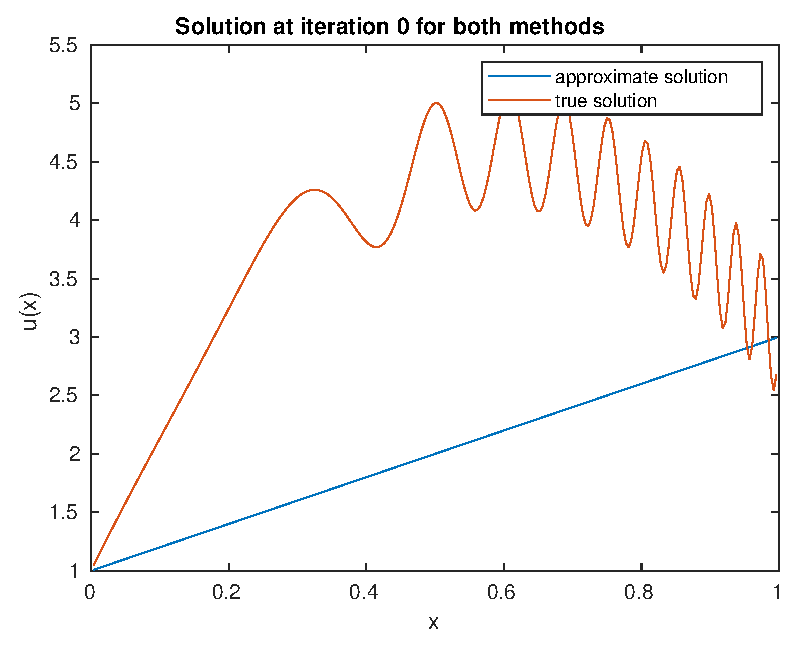
\includegraphics[width=\linewidth]{initial.eps}
    \end{subfigure}
    \begin{subfigure}{0.495\linewidth}
        \centering
        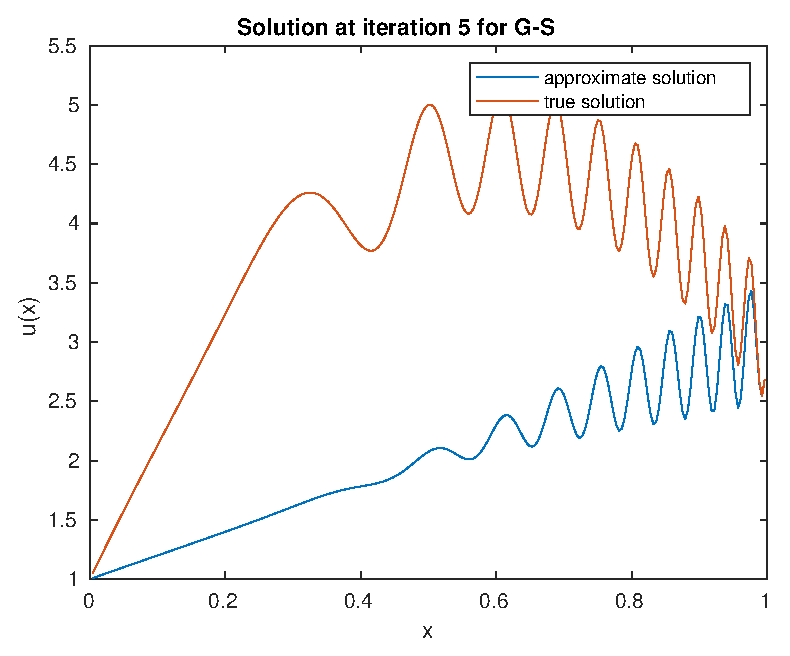
\includegraphics[width=\linewidth]{GS_i=5.eps}
    \end{subfigure}
    \begin{subfigure}{0.495\linewidth}
        \centering
        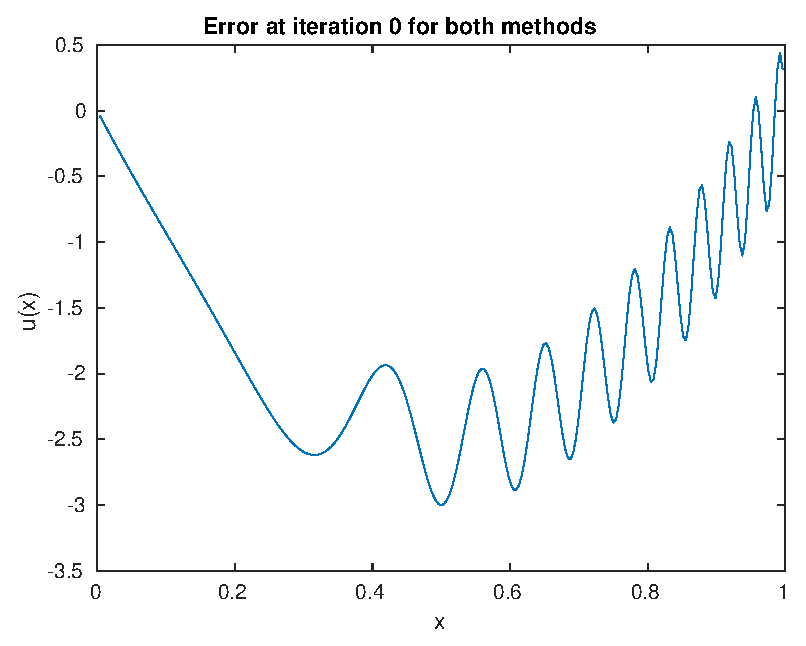
\includegraphics[width=\linewidth]{initialerr.eps}
    \end{subfigure}
    \begin{subfigure}{0.495\linewidth}
        \centering
        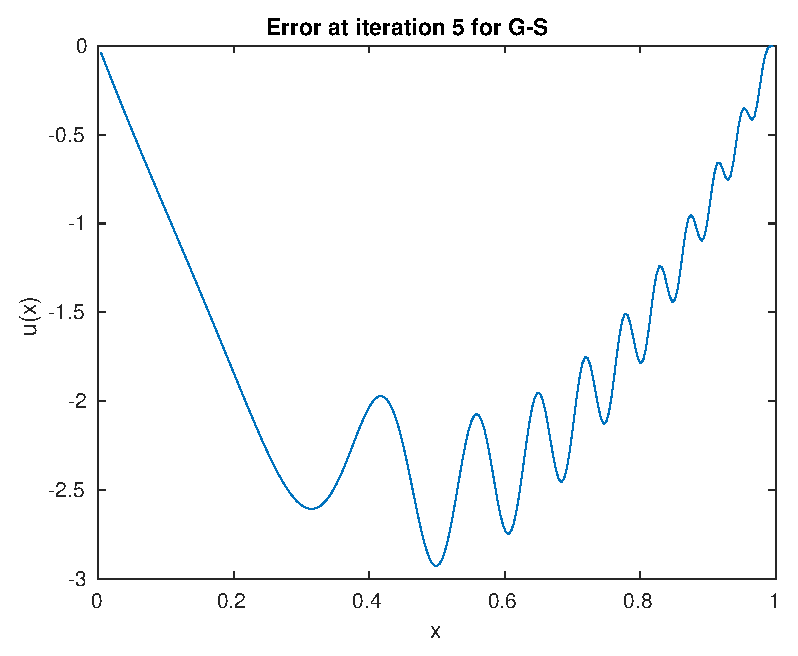
\includegraphics[width=\linewidth]{GSerr_i=5.eps}
    \end{subfigure}
\end{figure}
\begin{figure}[H]
    \centering
    \begin{subfigure}{0.495\linewidth}
        \centering
        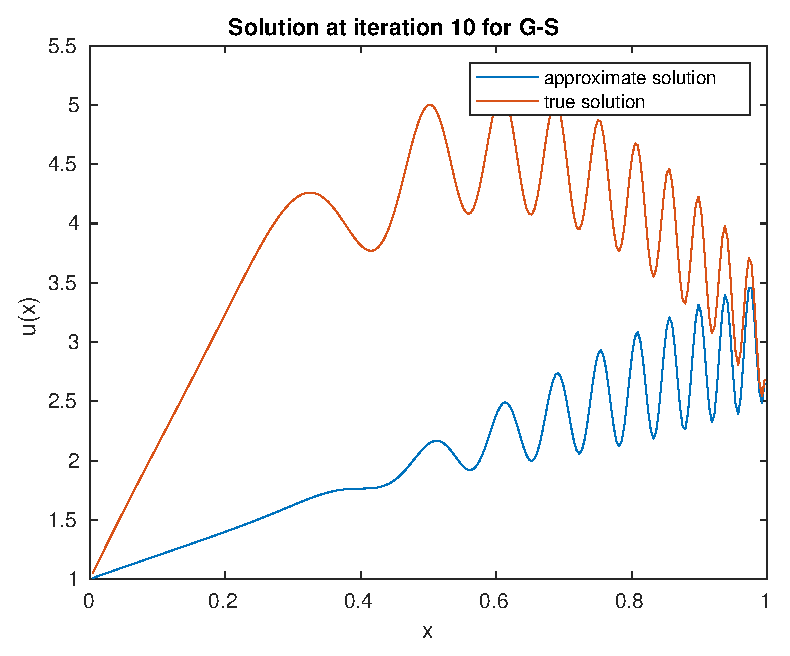
\includegraphics[width=\linewidth]{GS_i=10.eps}
    \end{subfigure}
    \begin{subfigure}{0.495\linewidth}
        \centering
        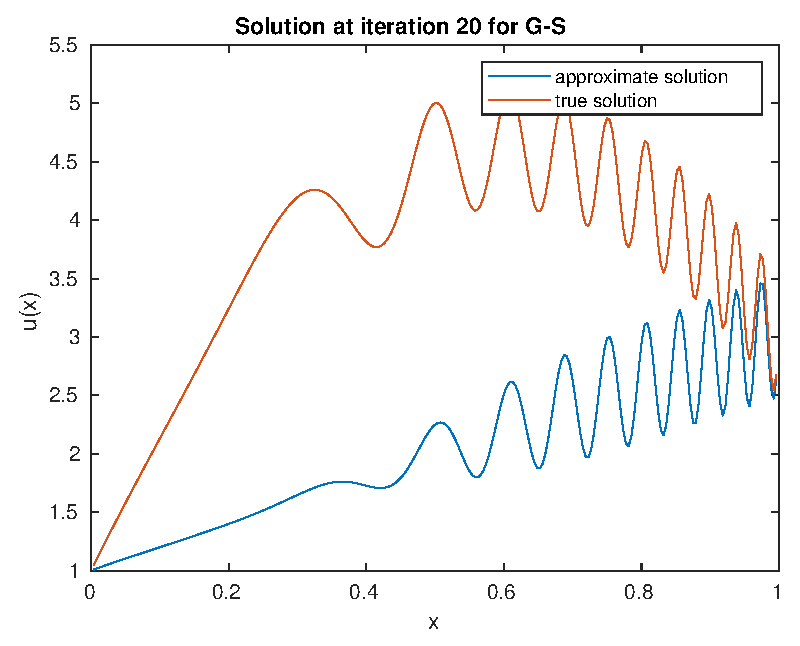
\includegraphics[width=\linewidth]{GS_i=20.eps}
    \end{subfigure}
    \begin{subfigure}{0.495\linewidth}
        \centering
        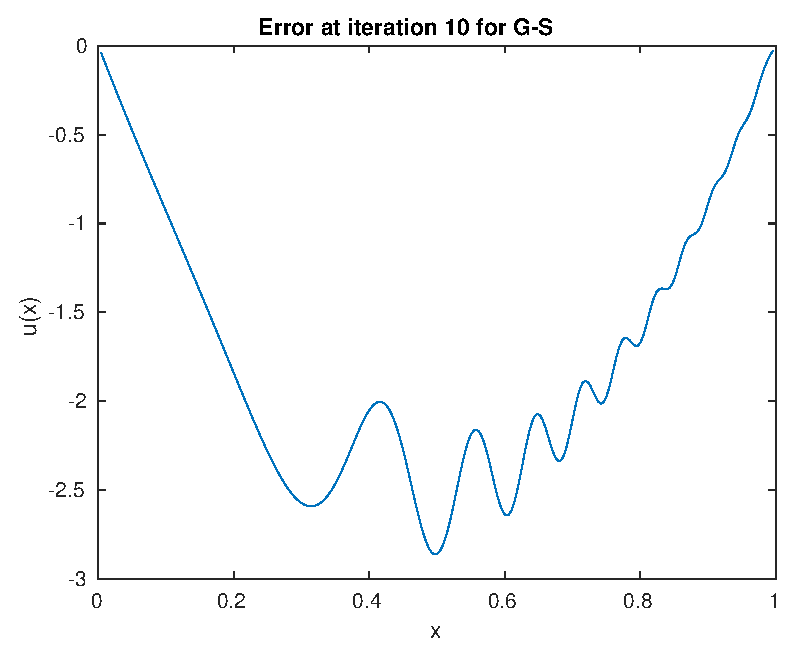
\includegraphics[width=\linewidth]{GSerr_i=10.eps}
    \end{subfigure}
    \begin{subfigure}{0.495\linewidth}
        \centering
        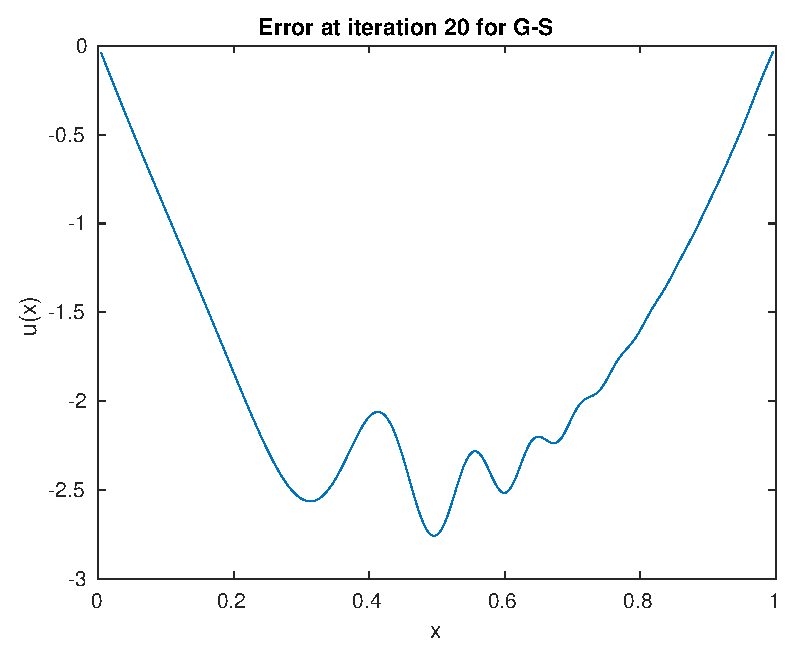
\includegraphics[width=\linewidth]{GSerr_i=20.eps}
    \end{subfigure}
\end{figure}
For conjugate gradient, we observe the following plots of our approximate solution and error relative to the true solution of the linear system at various iterations.\\
\begin{figure}[H]
    \centering
    \begin{subfigure}{0.495\linewidth}
        \centering
        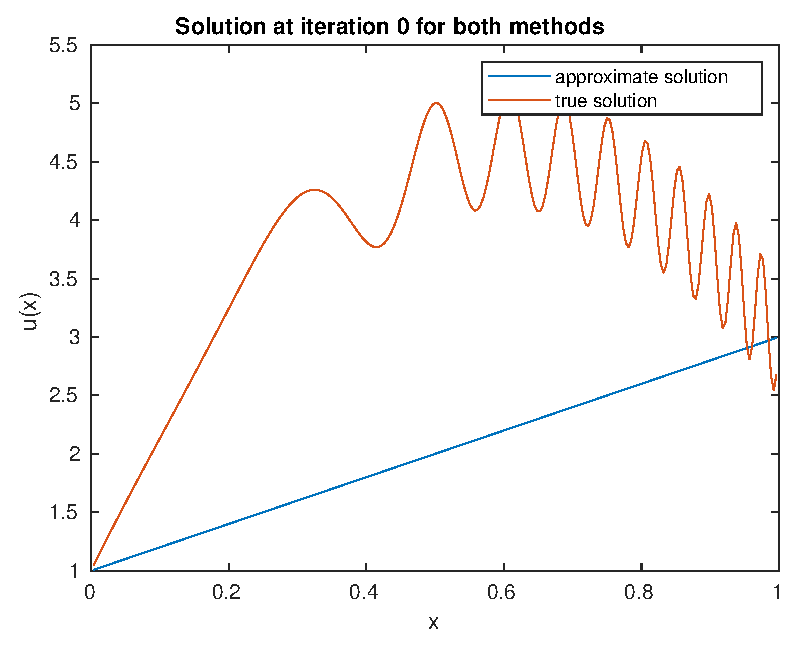
\includegraphics[width=\linewidth]{initial.eps}
    \end{subfigure}
    \begin{subfigure}{0.495\linewidth}
        \centering
        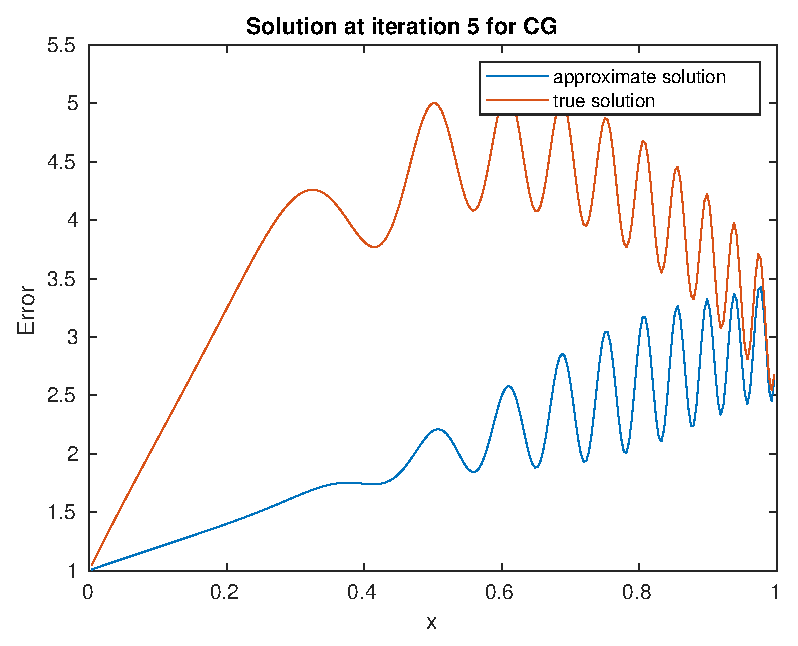
\includegraphics[width=\linewidth]{CG_i=5.eps}
    \end{subfigure}
    \begin{subfigure}{0.495\linewidth}
        \centering
        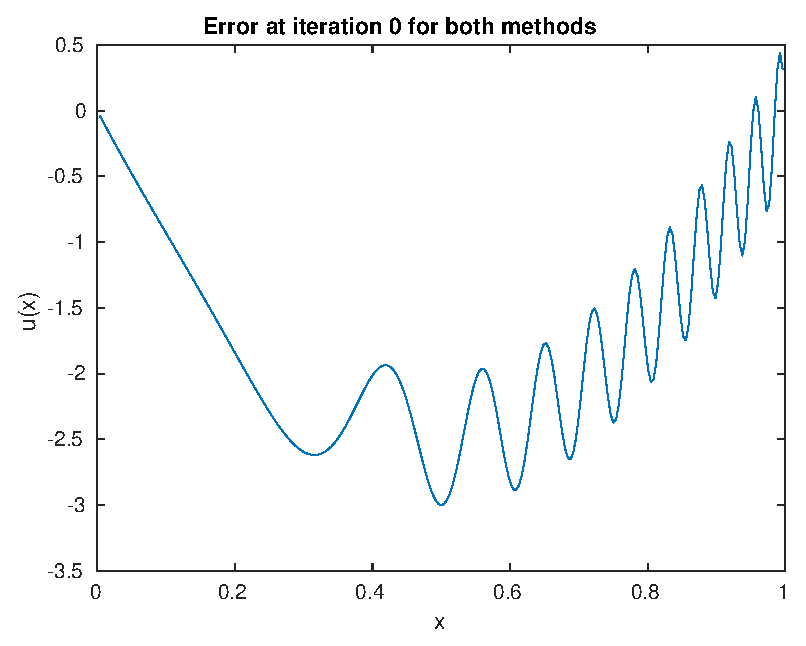
\includegraphics[width=\linewidth]{initialerr.eps}
    \end{subfigure}
    \begin{subfigure}{0.495\linewidth}
        \centering
        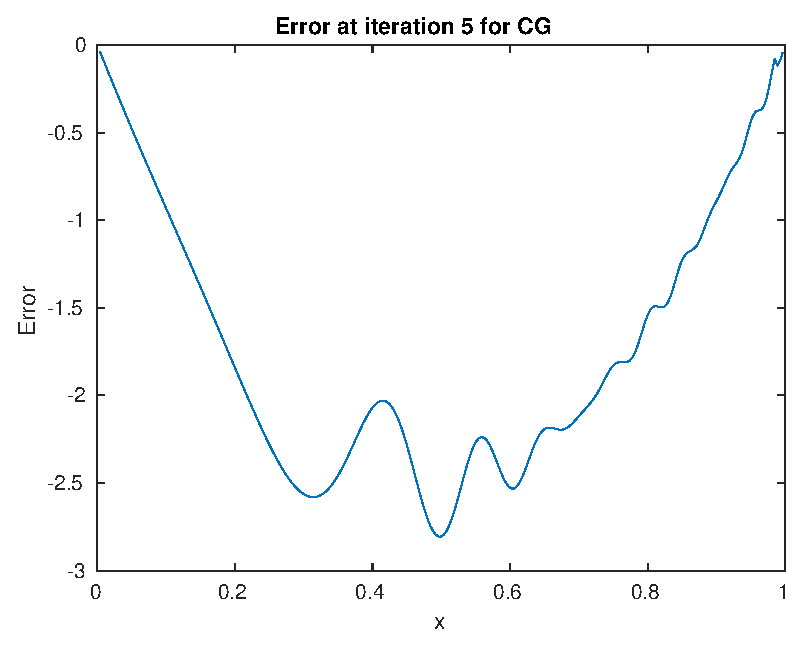
\includegraphics[width=\linewidth]{CGerr_i=5.eps}
    \end{subfigure}
    \begin{subfigure}{0.495\linewidth}
        \centering
        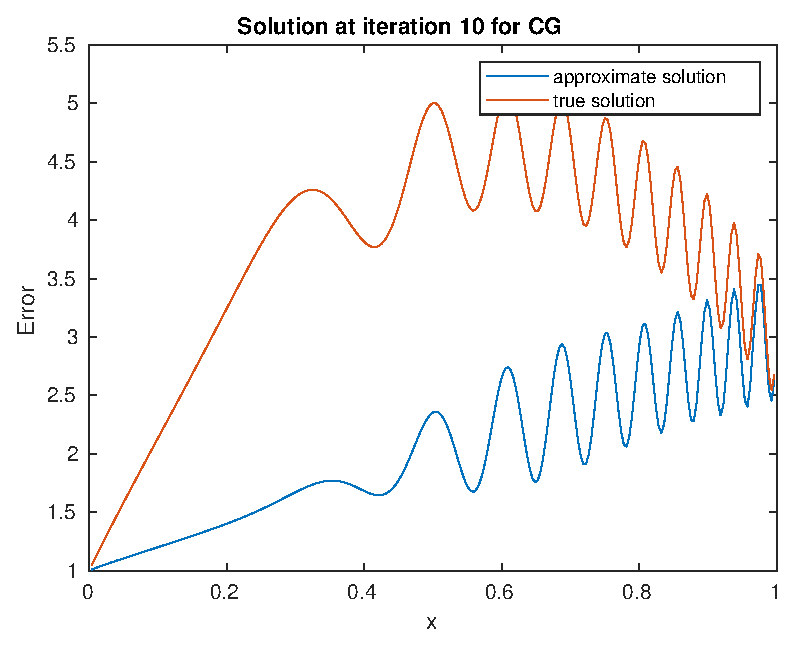
\includegraphics[width=\linewidth]{CG_i=10.eps}
    \end{subfigure}
    \begin{subfigure}{0.495\linewidth}
        \centering
        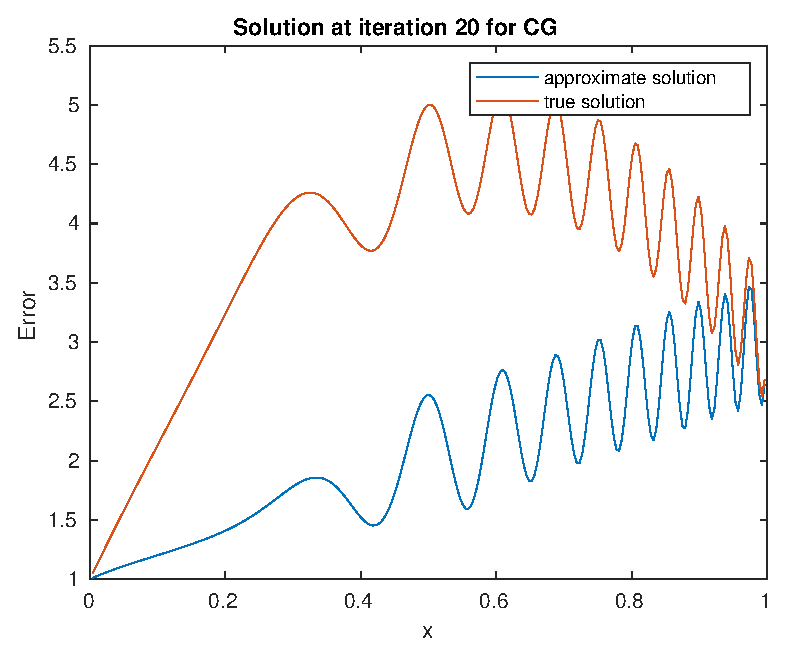
\includegraphics[width=\linewidth]{CG_i=20.eps}
    \end{subfigure}
    \begin{subfigure}{0.495\linewidth}
        \centering
        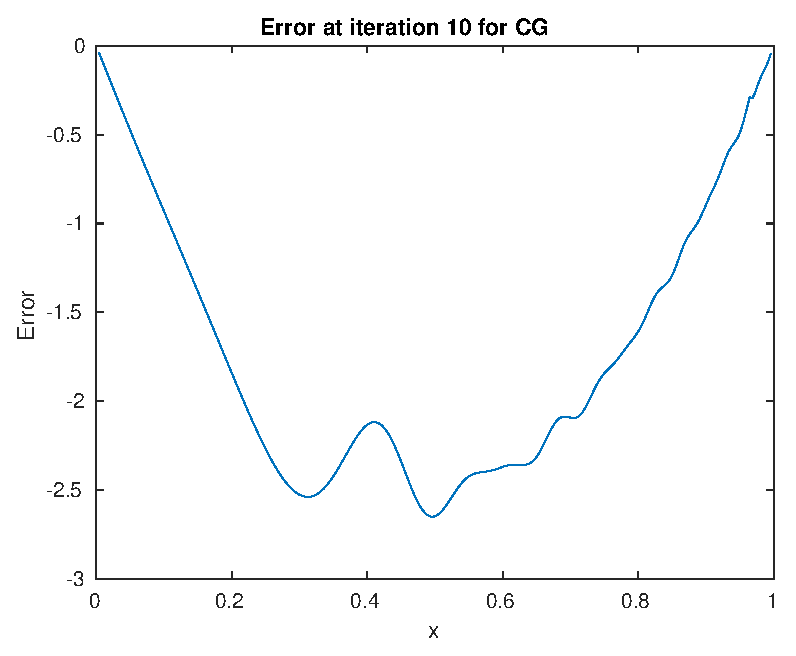
\includegraphics[width=\linewidth]{CGerr_i=10.eps}
    \end{subfigure}
    \begin{subfigure}{0.495\linewidth}
        \centering
        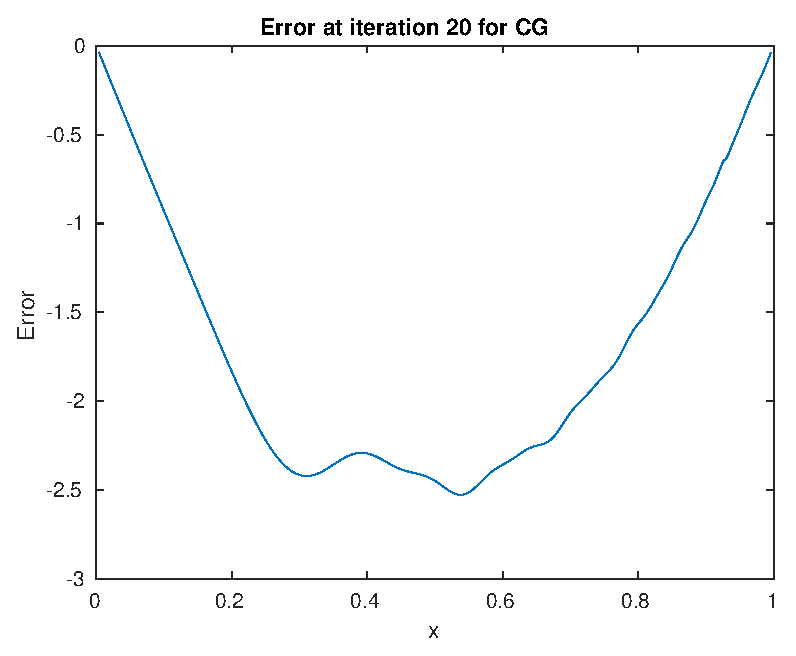
\includegraphics[width=\linewidth]{CGerr_i=20.eps}
    \end{subfigure}
\end{figure}
The following table gives the error in the infinity norm for each method.
\begin{table}[H]\centering
\begin{tabular}{|r|r|r|}\hline
{iteration}&{Conjugate Gradient}&{Gauss-Seidel}\\\hline
0&3.0015545862     &3.0015545862  \\
5&2.8056684895     &2.9260272297\\
10&2.6493059420&2.8612826923\\
20&2.5260624487&2.7575172522\\\hline
\end{tabular}
\end{table}
While both methods do a poor job of solving the linear system, they do appear to do a decent job of capturing the high-frequency portion of the true solution. Thus, they will likely make decent smoothers in spite of their poor performance overall.


\section{Problem 3}
Using MATLAB, we implement a 2-grid method for solving the 1D model problem with homogeneous Dirichlet
boundary conditions
\[
u_{xx} = f(x) ,~~u(0) = u(1) = 0.
\]
We use linear interpolation to go from the coarse grid with spacing $2h$ to the fine grid
with spacing $h$ and the projection matrix $I_h^{2h}$ going from the fine grid to the
coarse grid to be 
$I_h^{2h} = \frac{1}{2} ( I_{2h}^h )^T$ and se a multigrid V-cycle with 1 smoothing step on each visit to each grid level where both weighted Jacobi (with $\omega=2/3$) and Gauss-Seidel are used as the smoothing step in separate trials. For our function $f$, we use the same 
\[
f(x) = -20 + a \phi'' (x) \cos( \phi (x)) - a ( \phi' (x) )^2 \sin ( \phi (x) )
\]
from problem 2 but note that our boundary conditions now result in true solution
\[
u(x) = 1 + 12 x - 10 x^2 + a \sin ( \phi (x) ) -(2x+1).
\]
The following MATLAB code serves as our implementation.
\begin{verbatim}
phi = @(x) 20*pi*x.^3;
dphi = @(x) 60*pi*x.^2;
ddphi = @(x) 120*pi*x;
a = 1/2;
func = @(x) -20+a*ddphi(x).*cos(phi(x))-a*(dphi(x).^2).*sin(phi(x));
ufunc = @(x) 1+12*x-10*x.^2+a*sin(phi(x))-(1+2*x);

tol = 1e-13; maxiter=1000;

for m = [19 49 99 999]
    h = 1/(m+1); %need m odd here
    m_c = (m-1)/2; h_c = 2*h;
    x = linspace(0,1,m+2)';
    x = x(2:end-1);
    x_c = x(2:2:end);
    f = func(x); %randomly generate RHS vector


    % build FD matrix
    e = ones(m,1);
    A=spdiags([e -2*e e],[-1,0,1],m,m)/h^2;
    e_c = ones(m_c,1);
    A_c=spdiags([e_c -2*e_c e_c],[-1,0,1],m_c,m_c)/h_c^2;
    utrue = A\f;

    omega = 2/3; %suggested weight from class
    M = diag(diag(A))/omega; %weighted Jacobi

    u0 = zeros(size(utrue));

    [u,errvec,iter] = vcycle(A,f,A_c,M,u0,tol,maxiter);
    fprintf('Weighted Jacobi converged in %i iterations for h=%.2d.\n',iter,h)

    M=tril(A);
    [u,errvec,iter] = vcycle(A,f,A_c,M,u0,tol,maxiter);
    fprintf('Gauss-Seidel converged in %i iterations for h=%.2d.\n',iter,h)
end

function [u,resvec,iter] = vcycle(A,f,A_c,M,u0,tol,maxiter)
m = length(A);

e = ones(m,1);
Icf=spdiags([e/2 e e/2],[-1,0,1],m,m);
Icf = Icf(:,2:2:end);
Ifc = Icf'/2; 

r = f-A*u0;
u = u0; iter=0;
nf = norm(f); %save norm f
resnorm=norm(r)/nf; 
while resnorm>tol && iter<maxiter
    %beginning smoothing step
    u = u+M\r;
    r = f-A*u;

    r_c = Ifc*r;
    z_c = A_c\r_c;
    z = Icf*z_c;
    u = u+z;
    r = f-A*u;

    %ending smoothing step
    u = u+M\r;
    r = f-A*u;
    resnorm = norm(r)/nf;
    iter = iter+1;
    resvec(iter) = resnorm;
end

end
\end{verbatim}
We use a tolerance of $10^{-13}$ (near machine precision) for the relative residual and observe the following number of iterations required to converge to this tolerance for various values of $h$. 
\begin{table}[H]\centering
\begin{tabular}{|r|r|r|}\hline
{$h$}&{weighted Jacobi}&{Gauss-Seidel}\\\hline

0.05&14&14\\
0.02&14&15\\
0.01&14&15\\
0.001&15&15
\\\hline
\end{tabular}
\end{table}
Note that this is essentially constant with respect to $h$, so we achieve convergence to
a fixed tolerance in a number of cycles that is independent of the mesh size.

\section{Problem 4}
\subsection{Part a}
Consider an iteration of the form 
\[
x_k = x_{k-1} + M^{-1} ( b - A x_{k-1} ) ,
\]
for solving a nonsingular linear system $Ax=b$ and note that the error $e_k := A^{-1} b - x_k$
satisfies
\[
e_k = (I - M^{-1} A) e_{k-1} = \ldots = (I - M^{-1} A)^k e_0.
\]
If we assume that $\| e_0 \|_2 = 1$ and that $\| I - M^{-1} A \|_2 = \frac{1}{2}$, then by the properties of an operator norm,
\begin{align*}
\|e_k\|_2=\|(I - M^{-1} A)^k e_0\|_2\leq\|(I - M^{-1} A)\|^k_2\|e_0\|_2=2^{-k}. 
\end{align*}
Thus, we can guarantee that $\|e_k\|_2\leq 2^{-20}$ by taking $k=20$ iterations. If we instead have only that the spectral radius $\rho ( I - M^{-1} A ) = \frac{1}{2}$, we cannot give an estimate on the number of iterations
required to reduce the 2-norm of the error below $2^{-20}$. For a general square matrix $B$, its 2-norm is given by its largest singular value, but there is no way to bound this quantity by the spectral radius of $B$. Note that the inequality
\[
\sigma_{\text{min}}(B) \leq \min_{i}|\lambda_i|\leq\max_{i}|\lambda_i| \leq \sigma_{\text{max}}(B) 
\]
where the $\lambda$s denote the eigenvalues and the $\sigma$s denote the singular values holds, but there is no upper bound on $\sigma_{\text{max}}(B)$, so knowing the value of $\rho ( I - M^{-1} A )=\max_{i}|\lambda_i|$ gives only a lower bound on  $\|(I - M^{-1} A)\|_2=\sigma_{\text{max}}(B)$ which tells us nothing about convergence.

\subsection{Part b}
Now consider the GMRES algorithm applied to an $n$ by $n$ matrix $A$ with the sparsity pattern 
pictured below:
\[
\left[ \begin{array}{ccccc}
\ast & \ast & \cdots & \ast & \ast \\
\ast & \ast & \cdots & \ast & 0 \\
0    & \ast & \cdots & \ast & 0 \\
\vdots  & \ddots & \ddots & \vdots & \vdots \\
0    & \cdots    & \cdots & \ast & 0 \end{array} \right] ,
\]
where the $\ast$'s represent nonzero entries. Letting $\xi_j$ denote the $j$th unit vector, the algorithm makes no progress until step $n$ if the initial residual is $r_0=\xi_n$. Then, $Ar_0$ is a scalar multiple of $\xi_1$ (a linear combination of $\xi_1$) which in turn means that $A^2r_0$ is a linear combination of $\xi_1$ and $\xi_2$. We can continue this process to find that in general, $A^{k}r_0$ is a linear combination of $\xi_1,\ldots,\xi_k$. Thus, for $k=1,\ldots,n-1$, $A^{k}r_0$ is zero in its $n$th component, meaning that it must be orthogonal to $r_0=\xi_n$. This orthogonality poses a major issue. Fundamentally, GMRES seeks to find at each step
\[
r_k\in r_0+\Span\{Ar_0,\ldots,A^{k}r_0\}
\]
that minimizes $\|r_k\|^2$. However, we must have that $r_k=r_0$ for $k=1,\ldots,n-1$. Due to the orthogonality of all other vectors in this span to $r_0$, we cannot reduce the residual by including them in the linear combination that builds $x_k$ since they only contribute to the components aside from the last which are already zero. Of course, we can do at least as well as $r_0$ when adding more vectors to our span, so we must have that $r_k=r_0$ which means that $r_0=r_1=\ldots=r_{n-1}$. Thus, GMRES makes no progress until step $n$ at which it is guarenteed to solve the system.  \\
One form of a companion matrix is
\[
C=\left[ \begin{array}{ccccc}
-c_{n-1} & -c_{n-2} & \cdots & -c_{1} & -c_{0} \\
1 & 0 & \cdots & 0 & 0 \\
0    & 1 & \cdots & 0 & 0 \\
\vdots  & \ddots & \ddots & \vdots & \vdots \\
0    & \cdots    & \cdots & 1 & 0 \end{array} \right].
\]
It is well-known that the eigenvalues of $C$ are precisely the roots of the polynomial
\[
f(z)=z^n+\sum_{j=0}^{n-1}c_jz^j,
\]
but this is also easily seen by looking at $\lambda I-C$ and computing its determinant via expansion by minors on the first row to get characteristic equation
\[
0=\det(\lambda I-C)=\lambda^n+\sum_{j=0}^{n-1}c_j\lambda^j
\]
for the eigenvalues of $C$. However, we can always construct an $n$th degree monic polynomial that has $n$ roots $a_1,\ldots,a_n$ by considering $f(z)=(z-a_1)\cdots(z-a_n)$ and determining $c_1,\ldots,c_{n-1}$ by multiplying this product out. Thus, our equivalence means that we can construct a matrix $C$ that has any set of $n$ eigenvalues, meaning that companion matrices can have any eigenvalues. Note that companion matrices of this form have the sparsity pattern pictured above, meaning that matrices with that sparsity pattern can have any eigenvalues. This in conjunction with our earlier proof means that eigenvalue information alone cannot ensure that GMRES converges in less than $n$ iterations.

\end{document}